\PassOptionsToPackage{dvipsnames}{xcolor}
\documentclass{beamer}
\beamertemplatenavigationsymbolsempty
\usecolortheme{beaver}
\setbeamertemplate{blocks}[rounded=true, shadow=true]
\setbeamertemplate{footline}[page number]
% \usepackage[dvipsnames]{xcolor}

\usepackage[utf8]{inputenc}
\usepackage[english,russian]{babel}
\usepackage{amssymb,amsfonts,amsmath,mathtext}
\usepackage{algorithm}
\usepackage{algpseudocode}
\makeatletter
\renewcommand{\ALG@name}{Алгоритм}
\makeatother

\DeclareMathOperator*{\argmin}{arg\,min}
\DeclareMathOperator*{\argmax}{arg\,max}

%----------------------------------------------------------------------------------------------------------

\title[\hbox to 56mm{Адаптивное сжатие в распределенной оптимизации}]{Адаптивное сжатие в распределенной оптимизации}
\author[Ф.\,А.~Хафизов]{Фанис Адикович Хафизов\\
\small{Научный руководитель: к.ф.-м.н. А.\,Н.~Безносиков}}
\institute{Кафедра интеллектуальных систем ФПМИ МФТИ\\
Специализация: Интеллектуальный анализ данных\\
Направление: 03.03.01 Прикладные математика и физика}
\date{2024}

%----------------------------------------------------------------------------------------------------------

\begin{document}

%----------------------------------------------------------------------------------------------------------

\begin{frame}

    \maketitle

\end{frame}

%-----------------------------------------------------------------------------------------------------

\begin{frame}{Цель исследования}

    \textbf{Проблема:} Современные нейросети требуют больших вычислительных мощностей, из-за чего приходится прибегать к распределенным методам обучения.

    Одной из главных проблем является скорость передачи данных между устройствами.\\

    $ $\\

    \textbf{Цель:} Предложить новый способ сжатия градиентов для более эффективной коммуникации устройств.\\

    $ $\\

    \textbf{Решение:} Предлагается семейство смещенных операторов сжатия, использующие показатели важности весов.

\end{frame}

\begin{frame}{Литература}
    \begin{itemize}
     \item Aleksandr Beznosikov, Samuel Horváth, Peter Richtárik, Mher Safaryan. On Biased Compression for Distributed Learning. 2024
     \item Nam Nguyen, Deanna Needell, Tina Woolf. Linear Convergence of Stochastic Iterative Greedy Algorithms with Sparse Constraints. 2014
    \end{itemize}


\end{frame}

%-----------------------------------------------------------------------------------------------------

\begin{frame}{Постановка задачи}

    Ставится задача распределенной оптимизации.
    \begin{align*}
     \min_{x \in \mathbb{R}^d}\left\{f(x) := \frac{1}{n}\sum\limits_{i = 1}^n f_i(x) \right\},
    \end{align*}
    где $n$ -- количество устройств, $x$ -- обучаемые параметры, $f_i(x)$ -- функция потерь для $i$-го устройства.\\
    Требуется сократить количество передаваемой информации, не сильно потеряв в скорости обучения.

\end{frame}

%------------------------------------------------------------


%----------------------------------------------------------------------------------------------------------

\begin{frame}{Исследуемый метод}
    Для решения задачи распределенной оптимизации используется градиентный спуск со сжатием (DCGD)
    \begin{align*}
     x^{k + 1} = x^k - \frac{\eta}{n} \sum\limits_{i = 1}^n\mathcal{C}_i^k(\nabla f_i(x^k)),
    \end{align*}
    где $\eta$ -- размер шага, $\mathcal{C}_i^k$ -- оператор сжатия на $k$-й итерации $i$-го устройства.\\

    $ $\\
    Для случая одного устройства итерация метода запишется как
    \begin{align*}
     x^{k + 1} = x^k - \eta\mathcal{C}^k(\nabla f(x^k)).
    \end{align*}
\end{frame}

\begin{frame}{Исследуемый метод}
    Для еще большего сокращения размера передаваемой информации добавим оператор квантизации $\mathcal{Q}$.\\
    Метод DCGD тогда перепишется:
    \begin{align*}
     x^{k + 1} = x^k - \frac{\eta}{n} \sum\limits_{i = 1}^n \mathcal{Q}\left(\mathcal{C}_i^k(\nabla f_i(x^k))\right).
    \end{align*}
    Для одного устройства:
    \begin{align*}
     x^{k + 1} = x^k - \eta\mathcal{Q}\left(\mathcal{C}^k(\nabla f(x^k))\right).
    \end{align*}
    В качестве оператора $\mathcal{Q}$ выбрано округление до ближайшей степени 2.
\end{frame}

%----------------------------------------------------------------------------------------------------------

\begin{frame}{Базовое решение}
    В качестве базового решения рассматриваются операторы сжатия:
    \begin{itemize}
     \item RandK:
     \begin{align*}
      \mathcal{C}(x) := \frac{d}{k} \sum_{i \in S} x_i e_i,
     \end{align*}
     где $S \subseteq [d]$ -- случайный поднабор индексов размера $k$.
     \item TopK:
     \begin{align*}
      \mathcal{C}(x) := \frac{d}{k} \sum_{i = d - k + 1}^d x_{(i)} e_{(i)},
     \end{align*}
     где координаты расположены по неубыванию модуля $|x_{(1)}| \leq |x_{(2)}| \leq \dots \leq |x_{(d)}|$.
    \end{itemize}

\end{frame}

%----------------------------------------------------------------------------------------------------------

\begin{frame}{Предлагаемые операторы сжатия}
    Предлагается определить вектор важности $w \in [0, 1]^d$ и на основе  него построить семейство операторов сжатия $\mathcal{C}(x, w)$.\\
    $ $\\
    Для нахождения вектора $w$ решается задача оптимизации
    \begin{align*}
     w^k = \argmin_{w \in \Delta_d} f(x^k - \eta w \odot \nabla f(x^k)),
    \end{align*}
    где $\Delta_d = \left\{x \in \mathbb{R}^d ~|~ \sum\limits_{i = 1}^d x_i = 1, x_i \geq 0 ~ \forall i = \overline{1, d}\right\}$ -- вероятностный симплекс, $\odot$ -- поэлементное умножение.\\
    $ $\\
    Задача нахождения $w^k$ решается методом зеркального спуска на вероятностном симплексе.
\end{frame}

%----------------------------------------------------------------------------------------------------------

\begin{frame}{Примеры операторов сжатия с важностью}
    \begin{itemize}
     \item MD Stochastic
     \begin{align*}
      \mathcal{C}(x, w) := \frac{d}{k} \sum_{i \in S} x_i e_i,
     \end{align*}
     где $S \subseteq [d]$ -- случайный поднабор индексов размера $k$, вероятность выбора $i$-й компоненты равна $w_i$.
     \item MD Greedy
     \begin{align*}
      \mathcal{C}(x, w) := \frac{d}{k} \sum_{i = d - k + 1}^d x_{(i)} e_{(i)},
     \end{align*}
     где координаты расположены по неубыванию $w$: $w_{(1)} \leq w_{(2)} \leq \dots \leq w_{(d)}$.
    \end{itemize}
\end{frame}

\begin{frame}{Примеры операторов сжатия с важностью}
    \begin{itemize}
    \item MD Greedy Weighted
     \begin{align*}
      \mathcal{C}(x, w) := \frac{d}{k} \sum_{i = d - k + 1}^d w_{(i)} x_{(i)} e_{(i)},
     \end{align*}
     где координаты расположены по неубыванию $w$: $w_{(1)} \leq w_{(2)} \leq \dots \leq w_{(d)}$.

    \item MD Weighted Greedy
     \begin{align*}
      \mathcal{C}(x, w) := \frac{d}{k} \sum_{i = d - k + 1}^d w_{(i)} x_{(i)} e_{(i)},
     \end{align*}
     где координаты расположены по неубыванию взвешенных модулей: $|w_{(1)} x_{(1)}| \leq |w_{(2)} x_{(2)}| \leq \dots \leq |w_{(d)} x_{(d)}|$.
    \end{itemize}

\end{frame}

%----------------------------------------------------------------------------------------------------------


\begin{frame}{Эксперимент. Логистическая регрессия}

    \begin{figure}
     \centering
     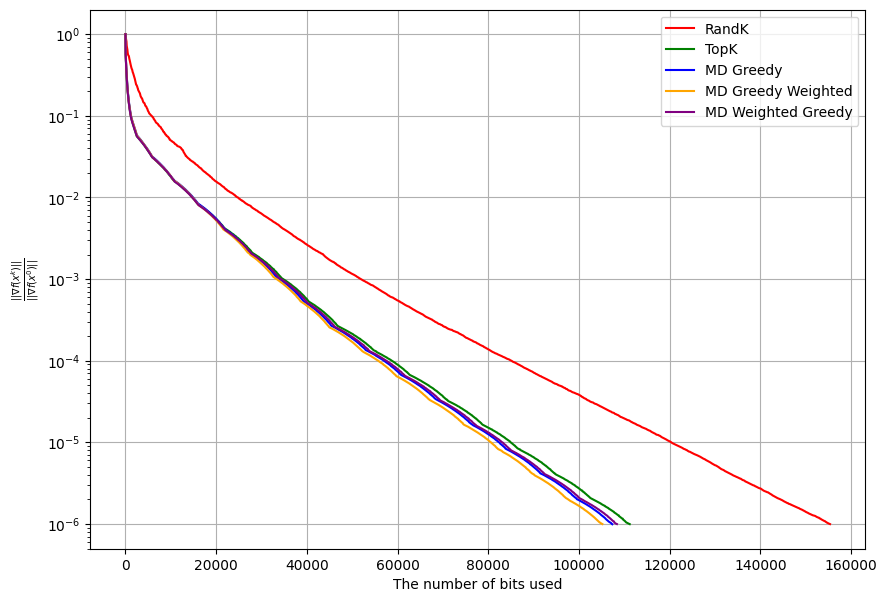
\includegraphics[width=0.9\textwidth]{../figures/LogReg}
     \caption{Сравнение операторов сжатия, задача логистической регрессии на датасете mushrooms, доля передаваемых компонент $k/d = 0.2$}
    \end{figure}

\end{frame}

%----------------------------------------------------------------------------------------------------------

\begin{frame}{Эксперимент. Классификация изображений}

    \begin{figure}
     \centering
     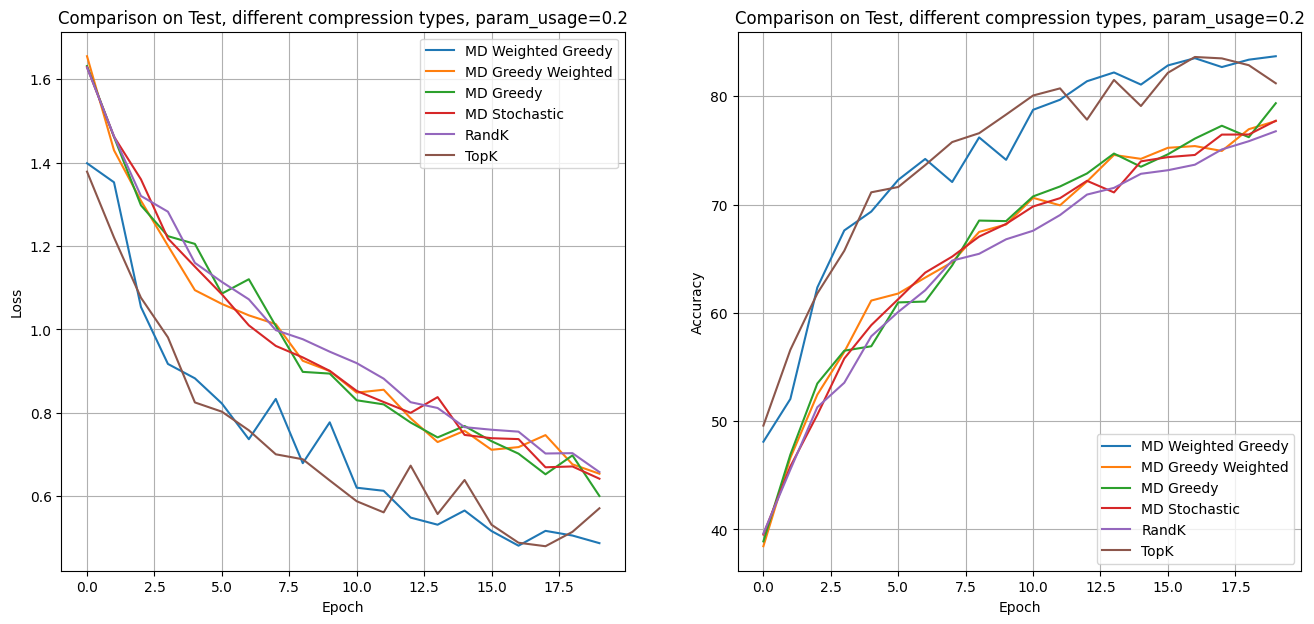
\includegraphics[width=\textwidth]{../figures/ResNet_CIFAR10}
     \caption{Сравнение операторов сжатия, задача классификации изображений на датасете CIFAR10, модель ResNet18, доля передаваемых компонент $k/d = 0.2$}
    \end{figure}

\end{frame}

%----------------------------------------------------------------------------------------------------------

\begin{frame}{Заключение}
    \begin{block}{Выносится на защиту}
    \begin{enumerate}
        \item Предложено семейство операторов сжатия, использующие вектор важности. Из него приведены 4 примера операторов.
        \item Вычислительные эксперименты показали, что предложенные операторы работают не хуже RandK, оператор MD Weighted Greedy работает на уровне TopK.
    \end{enumerate}
    \end{block}
    \begin{block}{Будущая работа}
    \begin{enumerate}
        \item Продолжать эксперименты, получить сходимость лучше TopK.
        \item Развить теорию для описанного семейства смещенных операторов.
    \end{enumerate}
    \end{block}

\end{frame}

%----------------------------------------------------------------------------------------------------------

\end{document}
